\subsection{Evaluating the forces using the Fast Multipole Method}
\label{ssec:fmm_summary}

The algorithmically challenging aspect of the \nbody problem is to
evaluate for each particle in a system the potential and associated
forces generated by all the other particles. Mathematically, this means
evaluate
\begin{equation}
  \phi(\mathbf{x}_a) = \sum_{b \neq a} G m_b\varphi(\mathbf{x}_a -
  \mathbf{x}_b)\qquad \forall~a\in N
  \label{eq:fmm:n_body}
\end{equation}
efficiently for large numbers of particles $N$. In the case of collisionless
dynamics, the particles are a mere Monte-Carlo sampling of the
underlying coarse-grained phase-space distribution which justifies the
use of approximate method to evaluate Eq.~\ref{eq:fmm:n_body}. The
\emph{Fast Multipole Method} (FMM) \citep{Greengard1987, Cheng1999},
popularized in the field and adapted specifically for gravity solvers
by \cite{Dehnen2000, Dehnen2002}, is an $\mathcal{O}(N)$ method
designed to solve Eq.~\ref{eq:fmm:n_body} by expanding the potential both
around $\mathbf{x}_i$ and $\mathbf{x}_j$ and grouping similar terms
arising from nearby particles. \\

In what follows, we use the compact multi-index notation of
\cite{Dehnen2014} (repeated in appendix \ref{sec:multi_index_notation}
for completeness) to simplify expressions and ease
comparisons. $\mathbf{k}$, $\mathbf{m}$ and $\mathbf{n}$ are
multi-indices and $\mathbf{r}$, $\mathbf{R}$, $\mathbf{x}$,
$\mathbf{y}$ and $\mathbf{z}$ are vectors, whilst $a$ and $b$ are
particle indices.\\

\begin{figure}
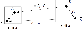
\includegraphics[width=\columnwidth]{cells.pdf}
\caption{The basics of the FMM: The potential generated by a particle
  at position $\mathbf{x}_b$ on a particle at position at location
  $\mathbf{x}_a$ is replaced by a Taylor expansion of the potential
  around the distance vector $\mathbf{R}$ linking the two centres of mass
  ($\mathbf{z}_A$ and $\mathbf{z}_B$) of cell $A$ and $B$. The
  expansion converges towards the exact expression provided
  $|\mathbf{R}|<|\mathbf{r}_a + \mathbf{r}_b|$.}
\label{fig:fmm:cells}
\end{figure}


For a single pair of particles $a$ and $b$ located in cell $A$ and $B$
with centres of mass $\mathbf{z}_A$ and  $\mathbf{z}_B$
respectively, as shown on Fig.~\ref{fig:fmm:cells}, the potential
generated by $b$ at the location of $a$ can be rewritten as
\begin{align}
  \varphi(\mathbf{x}_a - \mathbf{x}_b)
  &= \varphi\left(\mathbf{x}_a - \mathbf{z}_A - \mathbf{x}_b +
  \mathbf{z}_B + \mathbf{z}_A - \mathbf{z}_B\right)  \nonumber \\
  &= \varphi\left(\mathbf{r}_a - \mathbf{r}_b + \mathbf{R}\right)
  \nonumber \\
  &= \sum_\mathbf{k} \frac{1}{\mathbf{k}!} \left(\mathbf{r}_a -
  \mathbf{r}_b\right)^{\mathbf{k}} \nabla^{\mathbf{k}}\varphi(\mathbf{R})
  \nonumber \\
  &= \sum_\mathbf{k} \frac{1}{\mathbf{k}!} \sum_{\mathbf{n} <
    \mathbf{k}} \binom{\mathbf{k}}{\mathbf{n}} \mathbf{r}_a^{\mathbf{n}}
  \left(-\mathbf{r}_b\right)^{\mathbf{k} - \mathbf{n}}
  \nabla^{\mathbf{k}}\varphi(\mathbf{R})\nonumber \\
  &= \sum_\mathbf{n} \frac{1}{\mathbf{n}!} \mathbf{r}_a^{\mathbf{n}}
  \sum_\mathbf{m} \frac{1}{\mathbf{m}!}
  \left(-\mathbf{r}_b\right)^\mathbf{m} \nabla^{\mathbf{n}+\mathbf{m}} \varphi(\mathbf{R}),
\end{align}
where we used the Taylor expansion of $\varphi$ around $\mathbf{R} \equiv
\mathbf{z}_A - \mathbf{z}_B$ on the third line, used $\mathbf{r}_a
\equiv \mathbf{x}_a - \mathbf{z}_A$, $\mathbf{r}_b \equiv \mathbf{x}_b
- \mathbf{z}_B$ throughout and defined $\mathbf{m} \equiv
\mathbf{k}-\mathbf{n}$ on the last line. Expanding the series only up
to order $p$, we get
\begin{equation}
  \varphi(\mathbf{x}_a - \mathbf{x}_b) \approx \sum_{\mathbf{n}}^{p}
  \frac{1}{\mathbf{n}!} \mathbf{r}_a^{\mathbf{n}} \sum_{\mathbf{m}}^{p
    -|\mathbf{n}|} 
  \frac{1}{\mathbf{m}!} \left(-\mathbf{r}_b\right)^\mathbf{m}
  \nabla^{\mathbf{n}+\mathbf{m}} \varphi(\mathbf{R}),
  \label{eq:fmm:fmm_one_part}
\end{equation}
with the approximation converging as $p\rightarrow\infty$ towards the
correct value provided $|\mathbf{R}|<|\mathbf{r}_a +
\mathbf{r}_b|$. If we now consider all the particles within $B$ and
combine their contributions to the potential at location
$\mathbf{x}_a$ in cell $A$, we get
\begin{align}
  \phi_{BA}(\mathbf{x}_a) &= \sum_{b\in B}G m_b\varphi(\mathbf{x}_a -
  \mathbf{x}_b)  \label{eq:fmm:fmm_one_cell}  \\
  &\approx G\sum_{\mathbf{n}}^{p}
  \frac{1}{\mathbf{n}!} \mathbf{r}_a^{\mathbf{n}} \sum_{\mathbf{m}}
    ^{p -|\mathbf{n}|}
  \frac{1}{\mathbf{m}!} \sum_{b\in B} m_b\left(-\mathbf{r}_b\right)^\mathbf{m}
  \nabla^{\mathbf{n}+\mathbf{m}} \varphi(\mathbf{R}) \nonumber. 
\end{align}
This last equation forms the basis of the FMM. The algorithm
decomposes the equation into three separated sums evaluated at
different stages.\\

In a first step, multipoles are constructed from the
innermost sum. For each cell, we compute all the terms
\begin{equation}
  \mathsf{M}_{\mathbf{m}}(\mathbf{z}_B) = \frac{1}{\mathbf{m}!}
  \sum_{b\in B} m_b\left(-\mathbf{r}_b\right)^\mathbf{m} \label{eq:fmm:P2M} 
\end{equation}
up to order $p$. This is the first kernel of the method, commonly
labelled as \textsc{P2M} (particle to multipole). In a second step, we
compute the second kernel, \textsc{M2L} (multipole to local
expansion), which corresponds to the interaction of a cell with
another one:
\begin{equation}
  \mathsf{F}_{\mathbf{n}}(\mathbf{z}_A) = G\sum_{\mathbf{m}}^{p -|\mathbf{n}|}
  \mathsf{M}_{\mathbf{m}}(\mathbf{z}_B)
  \mathsf{D}_{\mathbf{n}+\mathbf{m}}(\mathbf{R}), \label{eq:fmm:M2L} 
\end{equation}
where $\mathsf{D}_{\mathbf{n}+\mathbf{m}}(\mathbf{R}) \equiv
\nabla^{\mathbf{n}+\mathbf{m}} \varphi(\mathbf{R})$ is an order $n+m$
derivative of the potential. This is the computationally expensive
step of the FMM algorithm as the number of operations in a naive
implementation using cartesian coordinates scales as
$\mathcal{O}(p^6)$. More advanced techniques
\citep[e.g.][]{Dehnen2014} can bring the cost down to
$\mathcal{O}(p^3)$, albeit at a considerable algebraic cost. For
collisionless dynamics, high accuracy is not required and low values
of $p$ are sufficient, which maintains the computational cost of the
M2L kernel at a reasonable level.  
Finally, in the last step, the potential is propagated from the local
expansion centre to the particles (L2P kernel) using
\begin{equation}
  \phi_{BA}(\mathbf{x}_a) = \sum_{\mathbf{n}}^{p}
  \frac{1}{\mathbf{n}!} \mathbf{r}_a^{\mathbf{n}}
  \mathsf{F}_{\mathbf{n}}(\mathbf{z}_A). \label{eq:fmm:L2P} 
\end{equation}
In summary, the potential generated by a cell $B$ on the particles in
cell $A$ is obtained by the successive application of the P2M, M2L and
L2P kernels. The P2M and L2P kernels are applied only once per
particle, whilst one M2L calculation has to be performed for each pair
of cells. The forces applied to the particles are obtained by the same
procedure using an extra order in the Taylor expansion. For instance,
for the acceleration along $x$, we have:
\begin{equation}
  a_x(\mathbf{x}_a) = \sum_{\mathbf{n}}^{p-1}
  \frac{1}{\mathbf{n}!} \mathbf{r}_a^{\mathbf{n}}
  \mathsf{F}_{\mathbf{n}+\left(1,0,0\right)}(\mathbf{z}_A). \label{eq:fmm:L2P_force} 
\end{equation}

In practice, the multipoles can be constructed recursively from the
leaves of the tree to the root and the local expansions from the root
to the leaves by shifting the $\mathsf{M}$ and $\mathsf{F}$ tensors
and adding their contributions to their parent or daughter cell's
tensors respecitvely. The shifting formulas (M2M and L2L kernels)
read:

\begin{align}
  \mathsf{M}_{\mathbf{m}}(\mathbf{x} + \mathbf{y}) &=
  \sum_{\mathbf{n}}^{\mathbf{m}}
  \frac{\mathbf{y}^\mathbf{n}}{\mathbf{n}!}\mathsf{M}_{\mathbf{m} -
    \mathbf{n}}(\mathbf{x}), \label{eq:fmm:M2M} \\
  \mathsf{F}_{\mathbf{n}}(\mathbf{x} + \mathbf{y}) &=
  \sum_{\mathbf{m}}^{p-|\mathbf{n}|}
  \frac{\mathbf{y}^\mathbf{m}}{\mathbf{m}!}\mathsf{F}_{\mathbf{m} +
    \mathbf{n}}(\mathbf{x}). \label{eq:fmm:L2L} 
\end{align}

All the kernels (Eqs.~\ref{eq:fmm:P2M}-\ref{eq:fmm:L2L}) are rather
straightforward to evaluate as they are only made of additions and
multiplications (provided $\mathsf{D}$ can be evaluated quickly),
which are extremely efficient instructions on modern
architectures. However, the fully expanded sums can lead to rather
large and prone to typo expressions. To avoid any mishaps, we use a
\texttt{python} script to generate C code in which all the sums are
unrolled and correct by construction. In \swift, we implemented the
kernels up to order $p=5$, as it proved to be accurate enough for our
purpose, but this could be extended to higher order easily. This
implies storing $56$ numbers per cell for each $\textsf{M}$ and
$\textsf{F}$ plus three numbers for the location of the centre of
mass. For leaf-cells with large numbers of particles, as in \swift,
this is a small memory overhead. One further small improvement
consists in choosing $\mathbf{z}_A$ to be the centre of mass of cell
$A$ rather than its geometrical centre. The first order multipoles
($\mathsf{M}_{100},\mathsf{M}_{010},\mathsf{M}_{001}$) then vanish by
construction. This allows us to simplify some of the expressions and
helps reduce, albeit by a small fraction, the memory footprint of the
tree structure.
